% Options for packages loaded elsewhere
\PassOptionsToPackage{unicode}{hyperref}
\PassOptionsToPackage{hyphens}{url}
\PassOptionsToPackage{dvipsnames,svgnames,x11names}{xcolor}
%
\documentclass[
  letterpaper,
  DIV=11,
  numbers=noendperiod]{scrartcl}

\usepackage{amsmath,amssymb}
\usepackage{iftex}
\ifPDFTeX
  \usepackage[T1]{fontenc}
  \usepackage[utf8]{inputenc}
  \usepackage{textcomp} % provide euro and other symbols
\else % if luatex or xetex
  \usepackage{unicode-math}
  \defaultfontfeatures{Scale=MatchLowercase}
  \defaultfontfeatures[\rmfamily]{Ligatures=TeX,Scale=1}
\fi
\usepackage{lmodern}
\ifPDFTeX\else  
    % xetex/luatex font selection
\fi
% Use upquote if available, for straight quotes in verbatim environments
\IfFileExists{upquote.sty}{\usepackage{upquote}}{}
\IfFileExists{microtype.sty}{% use microtype if available
  \usepackage[]{microtype}
  \UseMicrotypeSet[protrusion]{basicmath} % disable protrusion for tt fonts
}{}
\makeatletter
\@ifundefined{KOMAClassName}{% if non-KOMA class
  \IfFileExists{parskip.sty}{%
    \usepackage{parskip}
  }{% else
    \setlength{\parindent}{0pt}
    \setlength{\parskip}{6pt plus 2pt minus 1pt}}
}{% if KOMA class
  \KOMAoptions{parskip=half}}
\makeatother
\usepackage{xcolor}
\setlength{\emergencystretch}{3em} % prevent overfull lines
\setcounter{secnumdepth}{-\maxdimen} % remove section numbering
% Make \paragraph and \subparagraph free-standing
\makeatletter
\ifx\paragraph\undefined\else
  \let\oldparagraph\paragraph
  \renewcommand{\paragraph}{
    \@ifstar
      \xxxParagraphStar
      \xxxParagraphNoStar
  }
  \newcommand{\xxxParagraphStar}[1]{\oldparagraph*{#1}\mbox{}}
  \newcommand{\xxxParagraphNoStar}[1]{\oldparagraph{#1}\mbox{}}
\fi
\ifx\subparagraph\undefined\else
  \let\oldsubparagraph\subparagraph
  \renewcommand{\subparagraph}{
    \@ifstar
      \xxxSubParagraphStar
      \xxxSubParagraphNoStar
  }
  \newcommand{\xxxSubParagraphStar}[1]{\oldsubparagraph*{#1}\mbox{}}
  \newcommand{\xxxSubParagraphNoStar}[1]{\oldsubparagraph{#1}\mbox{}}
\fi
\makeatother

\usepackage{color}
\usepackage{fancyvrb}
\newcommand{\VerbBar}{|}
\newcommand{\VERB}{\Verb[commandchars=\\\{\}]}
\DefineVerbatimEnvironment{Highlighting}{Verbatim}{commandchars=\\\{\}}
% Add ',fontsize=\small' for more characters per line
\usepackage{framed}
\definecolor{shadecolor}{RGB}{241,243,245}
\newenvironment{Shaded}{\begin{snugshade}}{\end{snugshade}}
\newcommand{\AlertTok}[1]{\textcolor[rgb]{0.68,0.00,0.00}{#1}}
\newcommand{\AnnotationTok}[1]{\textcolor[rgb]{0.37,0.37,0.37}{#1}}
\newcommand{\AttributeTok}[1]{\textcolor[rgb]{0.40,0.45,0.13}{#1}}
\newcommand{\BaseNTok}[1]{\textcolor[rgb]{0.68,0.00,0.00}{#1}}
\newcommand{\BuiltInTok}[1]{\textcolor[rgb]{0.00,0.23,0.31}{#1}}
\newcommand{\CharTok}[1]{\textcolor[rgb]{0.13,0.47,0.30}{#1}}
\newcommand{\CommentTok}[1]{\textcolor[rgb]{0.37,0.37,0.37}{#1}}
\newcommand{\CommentVarTok}[1]{\textcolor[rgb]{0.37,0.37,0.37}{\textit{#1}}}
\newcommand{\ConstantTok}[1]{\textcolor[rgb]{0.56,0.35,0.01}{#1}}
\newcommand{\ControlFlowTok}[1]{\textcolor[rgb]{0.00,0.23,0.31}{\textbf{#1}}}
\newcommand{\DataTypeTok}[1]{\textcolor[rgb]{0.68,0.00,0.00}{#1}}
\newcommand{\DecValTok}[1]{\textcolor[rgb]{0.68,0.00,0.00}{#1}}
\newcommand{\DocumentationTok}[1]{\textcolor[rgb]{0.37,0.37,0.37}{\textit{#1}}}
\newcommand{\ErrorTok}[1]{\textcolor[rgb]{0.68,0.00,0.00}{#1}}
\newcommand{\ExtensionTok}[1]{\textcolor[rgb]{0.00,0.23,0.31}{#1}}
\newcommand{\FloatTok}[1]{\textcolor[rgb]{0.68,0.00,0.00}{#1}}
\newcommand{\FunctionTok}[1]{\textcolor[rgb]{0.28,0.35,0.67}{#1}}
\newcommand{\ImportTok}[1]{\textcolor[rgb]{0.00,0.46,0.62}{#1}}
\newcommand{\InformationTok}[1]{\textcolor[rgb]{0.37,0.37,0.37}{#1}}
\newcommand{\KeywordTok}[1]{\textcolor[rgb]{0.00,0.23,0.31}{\textbf{#1}}}
\newcommand{\NormalTok}[1]{\textcolor[rgb]{0.00,0.23,0.31}{#1}}
\newcommand{\OperatorTok}[1]{\textcolor[rgb]{0.37,0.37,0.37}{#1}}
\newcommand{\OtherTok}[1]{\textcolor[rgb]{0.00,0.23,0.31}{#1}}
\newcommand{\PreprocessorTok}[1]{\textcolor[rgb]{0.68,0.00,0.00}{#1}}
\newcommand{\RegionMarkerTok}[1]{\textcolor[rgb]{0.00,0.23,0.31}{#1}}
\newcommand{\SpecialCharTok}[1]{\textcolor[rgb]{0.37,0.37,0.37}{#1}}
\newcommand{\SpecialStringTok}[1]{\textcolor[rgb]{0.13,0.47,0.30}{#1}}
\newcommand{\StringTok}[1]{\textcolor[rgb]{0.13,0.47,0.30}{#1}}
\newcommand{\VariableTok}[1]{\textcolor[rgb]{0.07,0.07,0.07}{#1}}
\newcommand{\VerbatimStringTok}[1]{\textcolor[rgb]{0.13,0.47,0.30}{#1}}
\newcommand{\WarningTok}[1]{\textcolor[rgb]{0.37,0.37,0.37}{\textit{#1}}}

\providecommand{\tightlist}{%
  \setlength{\itemsep}{0pt}\setlength{\parskip}{0pt}}\usepackage{longtable,booktabs,array}
\usepackage{calc} % for calculating minipage widths
% Correct order of tables after \paragraph or \subparagraph
\usepackage{etoolbox}
\makeatletter
\patchcmd\longtable{\par}{\if@noskipsec\mbox{}\fi\par}{}{}
\makeatother
% Allow footnotes in longtable head/foot
\IfFileExists{footnotehyper.sty}{\usepackage{footnotehyper}}{\usepackage{footnote}}
\makesavenoteenv{longtable}
\usepackage{graphicx}
\makeatletter
\def\maxwidth{\ifdim\Gin@nat@width>\linewidth\linewidth\else\Gin@nat@width\fi}
\def\maxheight{\ifdim\Gin@nat@height>\textheight\textheight\else\Gin@nat@height\fi}
\makeatother
% Scale images if necessary, so that they will not overflow the page
% margins by default, and it is still possible to overwrite the defaults
% using explicit options in \includegraphics[width, height, ...]{}
\setkeys{Gin}{width=\maxwidth,height=\maxheight,keepaspectratio}
% Set default figure placement to htbp
\makeatletter
\def\fps@figure{htbp}
\makeatother

\usepackage{float}
\usepackage{tabularray}
\usepackage[normalem]{ulem}
\usepackage{graphicx}
\UseTblrLibrary{booktabs}
\UseTblrLibrary{rotating}
\UseTblrLibrary{siunitx}
\NewTableCommand{\tinytableDefineColor}[3]{\definecolor{#1}{#2}{#3}}
\newcommand{\tinytableTabularrayUnderline}[1]{\underline{#1}}
\newcommand{\tinytableTabularrayStrikeout}[1]{\sout{#1}}
\KOMAoption{captions}{tableheading}
\makeatletter
\@ifpackageloaded{caption}{}{\usepackage{caption}}
\AtBeginDocument{%
\ifdefined\contentsname
  \renewcommand*\contentsname{Table of contents}
\else
  \newcommand\contentsname{Table of contents}
\fi
\ifdefined\listfigurename
  \renewcommand*\listfigurename{List of Figures}
\else
  \newcommand\listfigurename{List of Figures}
\fi
\ifdefined\listtablename
  \renewcommand*\listtablename{List of Tables}
\else
  \newcommand\listtablename{List of Tables}
\fi
\ifdefined\figurename
  \renewcommand*\figurename{Figure}
\else
  \newcommand\figurename{Figure}
\fi
\ifdefined\tablename
  \renewcommand*\tablename{Table}
\else
  \newcommand\tablename{Table}
\fi
}
\@ifpackageloaded{float}{}{\usepackage{float}}
\floatstyle{ruled}
\@ifundefined{c@chapter}{\newfloat{codelisting}{h}{lop}}{\newfloat{codelisting}{h}{lop}[chapter]}
\floatname{codelisting}{Listing}
\newcommand*\listoflistings{\listof{codelisting}{List of Listings}}
\makeatother
\makeatletter
\makeatother
\makeatletter
\@ifpackageloaded{caption}{}{\usepackage{caption}}
\@ifpackageloaded{subcaption}{}{\usepackage{subcaption}}
\makeatother

\ifLuaTeX
  \usepackage{selnolig}  % disable illegal ligatures
\fi
\usepackage{bookmark}

\IfFileExists{xurl.sty}{\usepackage{xurl}}{} % add URL line breaks if available
\urlstyle{same} % disable monospaced font for URLs
\hypersetup{
  pdftitle={Homework 8},
  pdfauthor={Armin Bazarjani},
  colorlinks=true,
  linkcolor={blue},
  filecolor={Maroon},
  citecolor={Blue},
  urlcolor={Blue},
  pdfcreator={LaTeX via pandoc}}


\title{Homework 8}
\author{Armin Bazarjani}
\date{}

\begin{document}
\maketitle


\begin{Shaded}
\begin{Highlighting}[]
\FunctionTok{library}\NormalTok{(here)}
\FunctionTok{library}\NormalTok{(readxl)  }\CommentTok{\# for reading excel files}
\FunctionTok{library}\NormalTok{(modelsummary)  }\CommentTok{\# for summarizing data}
\FunctionTok{library}\NormalTok{(cmdstanr)  }\CommentTok{\# use two cores}
\FunctionTok{library}\NormalTok{(posterior)}
\FunctionTok{library}\NormalTok{(bayesplot)}
\FunctionTok{library}\NormalTok{(tidyverse)}
\FunctionTok{library}\NormalTok{(Lahman)}
\end{Highlighting}
\end{Shaded}

\section{Research Question}\label{research-question}

\begin{quote}
How does a player's batting ability change over their career?
\end{quote}

\section{Variables}\label{variables}

\begin{itemize}
\tightlist
\item
  \texttt{playerID}: Player ID Code
\item
  \texttt{yearID}: Year
\item
  \texttt{stint}: player's stint (order of appearances within a season)
\item
  \texttt{teamID}: Team; a factor
\item
  \texttt{H}: Number of hits in a season
\item
  \texttt{AB}: Number of at-bats in a season
\end{itemize}

\subsection{Data Import}\label{data-import}

\begin{Shaded}
\begin{Highlighting}[]
\FunctionTok{data}\NormalTok{(}\StringTok{"Batting"}\NormalTok{)}


\CommentTok{\# Data Processing Function}
\NormalTok{prepare\_batting\_data }\OtherTok{\textless{}{-}} \ControlFlowTok{function}\NormalTok{(batting\_data) \{}
\NormalTok{  batting\_processed }\OtherTok{\textless{}{-}}\NormalTok{ batting\_data }\SpecialCharTok{\%\textgreater{}\%}
    \CommentTok{\# Filter for sufficient at{-}bats (minimum 100 to be meaningful)}
    \FunctionTok{filter}\NormalTok{(AB }\SpecialCharTok{\textgreater{}=} \DecValTok{100}\NormalTok{) }\SpecialCharTok{\%\textgreater{}\%}
    \CommentTok{\# Calculate batting average}
    \FunctionTok{mutate}\NormalTok{(}\AttributeTok{BA =}\NormalTok{ H }\SpecialCharTok{/}\NormalTok{ AB) }\SpecialCharTok{\%\textgreater{}\%}
    \CommentTok{\# Group by player and calculate career year}
    \FunctionTok{group\_by}\NormalTok{(playerID) }\SpecialCharTok{\%\textgreater{}\%}
    \FunctionTok{arrange}\NormalTok{(yearID) }\SpecialCharTok{\%\textgreater{}\%}
    \FunctionTok{mutate}\NormalTok{(}
      \AttributeTok{career\_year =} \FunctionTok{row\_number}\NormalTok{(),}
      \CommentTok{\# Only keep players with at least 3 seasons}
      \AttributeTok{career\_length =} \FunctionTok{n}\NormalTok{()}
\NormalTok{    ) }\SpecialCharTok{\%\textgreater{}\%}
    \FunctionTok{filter}\NormalTok{(career\_length }\SpecialCharTok{\textgreater{}=} \DecValTok{3}\NormalTok{) }\SpecialCharTok{\%\textgreater{}\%}
    \FunctionTok{ungroup}\NormalTok{()}
  
  \FunctionTok{return}\NormalTok{(batting\_processed)}
\NormalTok{\}}

\NormalTok{processed\_data }\OtherTok{\textless{}{-}} \FunctionTok{prepare\_batting\_data}\NormalTok{(Batting)}

\CommentTok{\# Prepare data for a single player (Derek Jeter)}
\NormalTok{player\_data }\OtherTok{\textless{}{-}}\NormalTok{ processed\_data }\SpecialCharTok{\%\textgreater{}\%}
  \FunctionTok{filter}\NormalTok{(playerID }\SpecialCharTok{==} \StringTok{"jeterde01"}\NormalTok{)}
\end{Highlighting}
\end{Shaded}

\subsection{Variable Summary}\label{variable-summary}

\begin{Shaded}
\begin{Highlighting}[]
\FunctionTok{library}\NormalTok{(modelsummary)}

\FunctionTok{datasummary}\NormalTok{(}
\NormalTok{  BA }\SpecialCharTok{\textasciitilde{}}\NormalTok{ N }\SpecialCharTok{+}\NormalTok{ Mean }\SpecialCharTok{+}\NormalTok{ SD }\SpecialCharTok{+}\NormalTok{ Min }\SpecialCharTok{+}\NormalTok{ Max,}
  \AttributeTok{data =}\NormalTok{ player\_data,}
  \AttributeTok{output =} \StringTok{"markdown"}
\NormalTok{)}
\end{Highlighting}
\end{Shaded}

\begin{table}

\caption{\label{tbl-summ-var}Descriptive statistics of batting average
by career year}

\centering{

\centering
\begin{tblr}[         %% tabularray outer open
]                     %% tabularray outer close
{                     %% tabularray inner open
colspec={Q[]Q[]Q[]Q[]Q[]Q[]},
column{1}={}{halign=l,},
column{2,3,4,5,6}={}{halign=r,},
}                     %% tabularray inner close
\toprule
& N & Mean & SD & Min & Max \\ \midrule %% TinyTableHeader
BA & 18 & 0.31 & 0.02 & 0.26 & 0.35 \\
\bottomrule
\end{tblr}

}

\end{table}%

\section{Model}\label{model}

Model: \[
\begin{aligned}
H_i & \sim \text{Binomial}(AB_i, \theta_i) \\
\theta_i = \theta_{\text{base}} + \text{learning_rate} \times (Y_i - 1)
\end{aligned}
\]

Prior: \[
\begin{aligned}
\theta_{\text{base}} & \sim \text{Beta}(80, 240) \\
\text{learning_rate} & \sim N(0, 0.02) 
\end{aligned}
\]

\subsection{Analysis}\label{analysis}

I used 4 chains, each with 4,000 iterations (first 2,000 as warm-ups).

\section{Results}\label{results}

As shown in the rank histogram in Figure~\ref{fig-rank-hist-fit} below,
the chains mixed well.

\begin{Shaded}
\begin{Highlighting}[]
\FunctionTok{as\_draws}\NormalTok{(fit) }\SpecialCharTok{|\textgreater{}}
    \FunctionTok{mcmc\_rank\_hist}\NormalTok{(}\AttributeTok{pars =} \FunctionTok{c}\NormalTok{(}\StringTok{"theta\_base"}\NormalTok{, }\StringTok{"learning\_rate"}\NormalTok{))}
\end{Highlighting}
\end{Shaded}

\begin{figure}[H]

\centering{

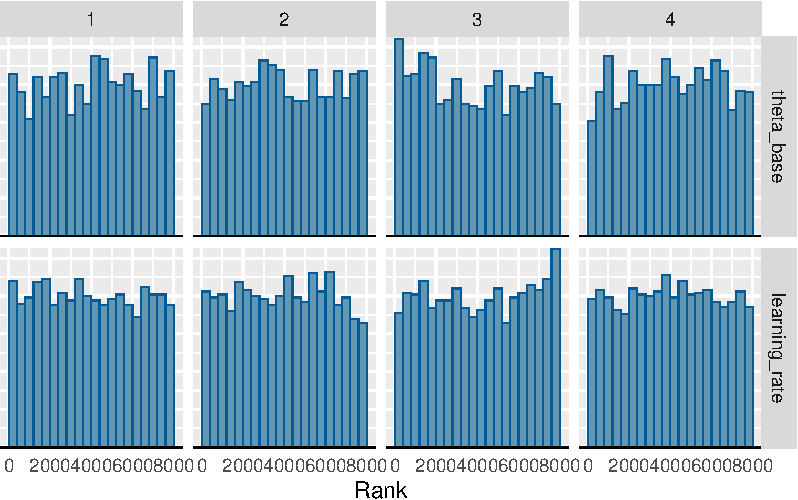
\includegraphics{hw8_BazarjaniArmin_files/figure-pdf/fig-rank-hist-fit-1.pdf}

}

\caption{\label{fig-rank-hist-fit}Rank histogram of the posterior
distributions of model parameters.}

\end{figure}%

Table~\ref{tbl-summ-fit} shows the posterior distributions of
\(\theta_{base}\) (base batting average), learning\_rate (yearly
change), and predicted batting averages for selected career years.

\begin{Shaded}
\begin{Highlighting}[]
\NormalTok{summ\_fit }\OtherTok{\textless{}{-}}\NormalTok{ fit}\SpecialCharTok{$}\FunctionTok{draws}\NormalTok{() }\SpecialCharTok{|\textgreater{}}
    \FunctionTok{subset\_draws}\NormalTok{(}\AttributeTok{variable =} \FunctionTok{c}\NormalTok{(}\StringTok{"theta\_base"}\NormalTok{, }\StringTok{"learning\_rate"}\NormalTok{, }\StringTok{"predicted\_ba[1]"}\NormalTok{, }\StringTok{"predicted\_ba[5]"}\NormalTok{, }\StringTok{"predicted\_ba[10]"}\NormalTok{)) }\SpecialCharTok{|\textgreater{}}
    \FunctionTok{rename\_variables}\NormalTok{(}
        \StringTok{"Base BA"} \OtherTok{=}\NormalTok{ theta\_base,}
        \StringTok{"Learning Rate"} \OtherTok{=}\NormalTok{ learning\_rate,}
        \StringTok{"Year 1 BA"} \OtherTok{=} \StringTok{\textasciigrave{}}\AttributeTok{predicted\_ba[1]}\StringTok{\textasciigrave{}}\NormalTok{,}
        \StringTok{"Year 5 BA"} \OtherTok{=} \StringTok{\textasciigrave{}}\AttributeTok{predicted\_ba[5]}\StringTok{\textasciigrave{}}\NormalTok{,}
        \StringTok{"Year 10 BA"} \OtherTok{=} \StringTok{\textasciigrave{}}\AttributeTok{predicted\_ba[10]}\StringTok{\textasciigrave{}}
\NormalTok{    ) }\SpecialCharTok{|\textgreater{}}
    \FunctionTok{summarise\_draws}\NormalTok{()}
\NormalTok{knitr}\SpecialCharTok{::}\FunctionTok{kable}\NormalTok{(summ\_fit, }\AttributeTok{digits =} \DecValTok{3}\NormalTok{)}
\end{Highlighting}
\end{Shaded}

\begin{longtable}[]{@{}
  >{\raggedright\arraybackslash}p{(\columnwidth - 18\tabcolsep) * \real{0.1818}}
  >{\raggedleft\arraybackslash}p{(\columnwidth - 18\tabcolsep) * \real{0.0909}}
  >{\raggedleft\arraybackslash}p{(\columnwidth - 18\tabcolsep) * \real{0.0909}}
  >{\raggedleft\arraybackslash}p{(\columnwidth - 18\tabcolsep) * \real{0.0779}}
  >{\raggedleft\arraybackslash}p{(\columnwidth - 18\tabcolsep) * \real{0.0779}}
  >{\raggedleft\arraybackslash}p{(\columnwidth - 18\tabcolsep) * \real{0.0909}}
  >{\raggedleft\arraybackslash}p{(\columnwidth - 18\tabcolsep) * \real{0.0779}}
  >{\raggedleft\arraybackslash}p{(\columnwidth - 18\tabcolsep) * \real{0.0779}}
  >{\raggedleft\arraybackslash}p{(\columnwidth - 18\tabcolsep) * \real{0.1169}}
  >{\raggedleft\arraybackslash}p{(\columnwidth - 18\tabcolsep) * \real{0.1169}}@{}}

\caption{\label{tbl-summ-fit}Posterior summary of the model parameters.}

\tabularnewline

\toprule\noalign{}
\begin{minipage}[b]{\linewidth}\raggedright
variable
\end{minipage} & \begin{minipage}[b]{\linewidth}\raggedleft
mean
\end{minipage} & \begin{minipage}[b]{\linewidth}\raggedleft
median
\end{minipage} & \begin{minipage}[b]{\linewidth}\raggedleft
sd
\end{minipage} & \begin{minipage}[b]{\linewidth}\raggedleft
mad
\end{minipage} & \begin{minipage}[b]{\linewidth}\raggedleft
q5
\end{minipage} & \begin{minipage}[b]{\linewidth}\raggedleft
q95
\end{minipage} & \begin{minipage}[b]{\linewidth}\raggedleft
rhat
\end{minipage} & \begin{minipage}[b]{\linewidth}\raggedleft
ess\_bulk
\end{minipage} & \begin{minipage}[b]{\linewidth}\raggedleft
ess\_tail
\end{minipage} \\
\midrule\noalign{}
\endhead
\bottomrule\noalign{}
\endlastfoot
Base BA & 0.318 & 0.318 & 0.008 & 0.008 & 0.304 & 0.331 & 1.002 &
1817.731 & 1693.568 \\
Learning Rate & -0.001 & -0.001 & 0.001 & 0.001 & -0.002 & 0.000 & 1.001
& 2254.289 & 2275.201 \\
Year 1 BA & 0.318 & 0.318 & 0.008 & 0.008 & 0.304 & 0.331 & 1.002 &
1817.731 & 1693.568 \\
Year 5 BA & 0.313 & 0.314 & 0.006 & 0.006 & 0.304 & 0.323 & 1.002 &
2006.224 & 2137.741 \\
Year 10 BA & 0.308 & 0.308 & 0.004 & 0.004 & 0.301 & 0.315 & 1.000 &
5522.569 & 5170.544 \\

\end{longtable}

Figure~\ref{fig-career-trajectory} shows the model's estimates of the
player's (Derek Jeter) career batting trajectory

\begin{Shaded}
\begin{Highlighting}[]
\CommentTok{\#| label: fig{-}career{-}trajectory}
\CommentTok{\#| fig{-}cap: Career batting average trajectory with 90\% credible intervals}

\CommentTok{\# Extract posterior predictions and create proper data frame}
\NormalTok{draws }\OtherTok{\textless{}{-}}\NormalTok{ fit}\SpecialCharTok{$}\FunctionTok{draws}\NormalTok{(}\StringTok{"predicted\_ba"}\NormalTok{)}
\NormalTok{pred\_df }\OtherTok{\textless{}{-}} \FunctionTok{data.frame}\NormalTok{(}
  \AttributeTok{year =} \DecValTok{1}\SpecialCharTok{:}\DecValTok{18}\NormalTok{,  }\CommentTok{\# Explicitly use 18 years}
  \AttributeTok{mean =} \FunctionTok{apply}\NormalTok{(draws, }\DecValTok{3}\NormalTok{, mean),}
  \AttributeTok{lower =} \FunctionTok{apply}\NormalTok{(draws, }\DecValTok{3}\NormalTok{, }\ControlFlowTok{function}\NormalTok{(x) }\FunctionTok{quantile}\NormalTok{(x, }\FloatTok{0.05}\NormalTok{)),}
  \AttributeTok{upper =} \FunctionTok{apply}\NormalTok{(draws, }\DecValTok{3}\NormalTok{, }\ControlFlowTok{function}\NormalTok{(x) }\FunctionTok{quantile}\NormalTok{(x, }\FloatTok{0.95}\NormalTok{))}
\NormalTok{)}

\CommentTok{\# Plot}
\FunctionTok{ggplot}\NormalTok{() }\SpecialCharTok{+}
    \CommentTok{\# Add shaded credible interval}
    \FunctionTok{geom\_ribbon}\NormalTok{(}\AttributeTok{data =}\NormalTok{ pred\_df,}
                \FunctionTok{aes}\NormalTok{(}\AttributeTok{x =}\NormalTok{ year, }\AttributeTok{ymin =}\NormalTok{ lower, }\AttributeTok{ymax =}\NormalTok{ upper),}
                \AttributeTok{fill =} \StringTok{"lightblue"}\NormalTok{, }\AttributeTok{alpha =} \FloatTok{0.3}\NormalTok{) }\SpecialCharTok{+}
    \CommentTok{\# Add mean prediction line}
    \FunctionTok{geom\_line}\NormalTok{(}\AttributeTok{data =}\NormalTok{ pred\_df,}
              \FunctionTok{aes}\NormalTok{(}\AttributeTok{x =}\NormalTok{ year, }\AttributeTok{y =}\NormalTok{ mean),}
              \AttributeTok{color =} \StringTok{"blue"}\NormalTok{) }\SpecialCharTok{+}
    \CommentTok{\# Add actual observed batting averages}
    \FunctionTok{geom\_point}\NormalTok{(}\AttributeTok{data =}\NormalTok{ player\_data,}
               \FunctionTok{aes}\NormalTok{(}\AttributeTok{x =}\NormalTok{ career\_year, }\AttributeTok{y =}\NormalTok{ BA)) }\SpecialCharTok{+}
    \CommentTok{\# Labels and theme}
    \FunctionTok{labs}\NormalTok{(}\AttributeTok{x =} \StringTok{"Career Year"}\NormalTok{,}
         \AttributeTok{y =} \StringTok{"Batting Average"}\NormalTok{,}
         \AttributeTok{title =} \StringTok{"Career Batting Average Trajectory"}\NormalTok{) }\SpecialCharTok{+}
    \CommentTok{\# Set y{-}axis limits based on the data}
    \FunctionTok{scale\_y\_continuous}\NormalTok{(}\AttributeTok{limits =} \FunctionTok{c}\NormalTok{(}\FloatTok{0.25}\NormalTok{, }\FloatTok{0.36}\NormalTok{), }
                      \AttributeTok{breaks =} \FunctionTok{seq}\NormalTok{(}\FloatTok{0.25}\NormalTok{, }\FloatTok{0.36}\NormalTok{, }\FloatTok{0.02}\NormalTok{)) }\SpecialCharTok{+}
    \FunctionTok{theme\_minimal}\NormalTok{()}
\end{Highlighting}
\end{Shaded}

\begin{figure}[H]

\centering{

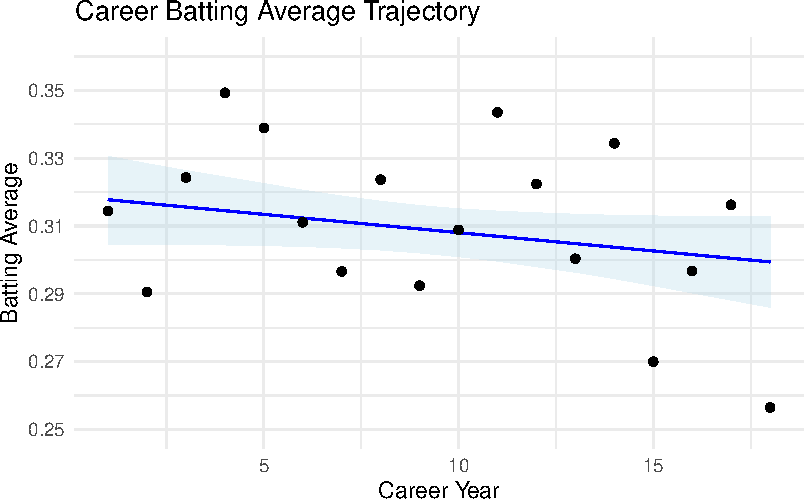
\includegraphics{hw8_BazarjaniArmin_files/figure-pdf/fig-career-trajectory-1.pdf}

}

\caption{\label{fig-career-trajectory}Career batting average trajectory
with 90\% credible intervals}

\end{figure}%

\section{Future Plans}\label{future-plans}

After doing this initial analysis there are a few things I think that I
would like to do: 1. I could try using a non-linear learning rate
between seasons. 2. Try non-linear models for modeling career batting
averages 3. Add covariates, things like age, position, ballpark, etc. 4.
I would like to try a hierarchical model.




\end{document}
